\chapter{Ordinary Differential Equations}

\vspace*{-1cm}
\begin{flushright}
\texttt{ENIAC, since 1946}
\end{flushright}

\lettrine[nindent=0.35em,lhang=0.40,loversize=0.3]{E}{NIAC}, \textbf{E}lectronic \textbf{N}umerical \textbf{I}ntegrator \textbf{A}nd \textbf{C}omputer\cite{haigh2016eniac},
the first electronic general-purpose computer was designed by the US Army and finished in 1946\footnote{ENIAC: \url{https://en.wikipedia.org/wiki/ENIAC}}. The goal was to numerically calculate artillery firing tables by solving sets of differential equations. Essentially, $\bm{F} = m\bm{a}$ with quite a few complications.

Indeed we are surrounded by differential equations...

\begin{equation}
 m \dfrac{\partial^2 \bm{r}}{\partial t^2} = \bm{F},
\end{equation}

\begin{equation}
 i\hbar \dfrac{\partial \psi(\bm{r},t)}{\partial t} = H \psi(\bm{r},t),
\end{equation}

\begin{equation}
 \begin{array}{c c c c}
  \bm{\nabla}\cdot\bm{D} = \rho, \quad & \bm{\nabla}\cdot\bm{B} = 0, \quad & \bm{\nabla}\times\bm{E} = -\dfrac{\partial \bm{B}}{\partial t}, \quad & \bm{\nabla}\times\bm{H} = \dfrac{\partial \bm{D}}{\partial t} + \bm{J},
 \end{array}
\end{equation}

\begin{equation}
 \dfrac{\partial u}{\partial t} -\alpha^2 \bm{\nabla}^2 u = 0,
\end{equation}

\begin{equation}
 \dfrac{\partial^2 u}{\partial t^2} - c^2 \bm{\nabla}^2 u = 0,
\end{equation}

... to list a few. We also have Navier–Stokes, general relativity, etc.

The unknown quantity in a differential equation can be a function of a single variable, like the position that depends on time on Newton's second law above ($\bm{r} \equiv \bm{r}(t)$). These cases are labeled \texttt{ordinary differential equations} (ODE). If your function depends upon two or more variables and your differential equation has derivatives on these variables, it becomes a \texttt{partial differential equation} (PDE). This is the case of all other examples above. PDEs and ODEs are intrinsically different. Important theorems of ODEs do not apply for PDEs.

Let us compare two simple cases, the Laplace equation in one and two dimensions:

\begin{align}
 \dfrac{\partial^2 f(x)}{\partial x^2} &= 0,\\
 \left(\dfrac{\partial^2}{\partial x^2} + \dfrac{\partial^2}{\partial y^2}\right)f(x,y) &= 0.
\end{align}

The 1D equation is a second order ODE. This means that its most general solution is defined up to two unknown constants. These are set by two initial or boundary conditions. In this case the general solution is a straight line,

\begin{equation}
 f(x) = c_1x + c_0,
\end{equation}
where $c_1$ and $c_0$ are the unknown coefficients.

Contrasting the simplicity of the 1D Laplace equation, the 2D version, which is a PDE, has an infinite number of solutions. Introducing complex variables, it is easy to verify that the most general solution is

\begin{equation}
 f(x,y) = p(z) + q(\bar{z}),
\end{equation}
where $p(z)$, $q(\bar{z})$ are arbitrary analytical functions of the complex variables $z = x+iy$, $\bar{z} = x-iy$.

For now, we will focus on \texttt{ordinary differential equations} (ODE). These can be classified into three main categories: (i) initial value problems; (ii) boundary-value problems; and (iii) eigenvalue problems. Here we shall restrict ourselves to introductory discussion on the methods to solve ODEs, for more details please check Ref.~\cite{JCButcher2008NumericalODE, pang2006introduction}.


\section{Initial value problem: time-evolution}

Initial value problems usually deal with the dynamics of a system, where the derivatives are taken with respect to time. Newton's second law is the paradigmatic example of an initial value ODE,

\begin{equation}
 \dfrac{d^2 \bm{r}}{dt^2} = \dfrac{\bm{F}}{m},
\end{equation}
requiring the \texttt{initial} position $\bm{r}(0)$ and velocity $\bm{v}(0)$ to be solved.

Let's consider the one dimensional case to guide our discussion. Just keep in mind that a generalization to more dimensions is immediate. First we write Newton's second law in a more general form of an arbitrary second order initial value problem ODE,

\begin{equation}
 \dfrac{d^2 x}{dt^2} = g(x,t).
\end{equation}

This second order ODE can be split into a pair of coupled first order ODEs using $v = \frac{dx}{dt}$, yielding

\begin{equation}
 \dfrac{dv}{dt} = g(x,t), \quad \text{ and } \quad \dfrac{dx}{dt} = v.
\end{equation}

Finally, we can define vectors $\bm{y} = [ v(t), x(t) ]$ and $\bm{f} = [ g(x,t), v(t) ]$, such that the equations above can be cast as

\begin{equation}
 \dfrac{d \bm{y}}{dt} = \bm{f}.
 \label{eq:dydteqf}
\end{equation}


\subsection*{Example: the pendulum}

Any physics text-book will tell you that the equation of motion for the pendulum is

\begin{equation}
 \dfrac{d^2\theta(t)}{dt^2} = -\omega^2 \sin[\theta(t)],
 \label{eq:pendulum}
\end{equation}
where $\theta(t)$ is the angular displacement, $\omega^2 = g/\ell$, $g \approx 9.8$~m/s$^s$ is the gravity, and $\ell$ is the pendulum length.

For small oscillations we can use Taylor's expansion to write $\sin\theta \approx \theta$. This leads to the usual harmonic solution $\theta(t) = A\cos(\omega t + \phi)$, where the amplitude $A$ and the phase constant $\phi$ are set by initial conditions.

Let us try to go beyond the small oscillations approximation and numerically solve Eq.~\eqref{eq:pendulum} with the content of the next sections. To do this, first we have to rewrite Eq.~\eqref{eq:pendulum} in the form of a set of coupled first order ODEs as we generically did above. With this purpose, define\footnote{Within the text I'll use the dot notation to refer to time derivatives, \textit{i.e.} $\dot{\theta} = \dfrac{d\theta}{dt}$} $x(t) = \theta(t)$ and $v(t) = \dot{\theta}(t)$. The pendulum equation of motion becomes

\begin{equation}
 \dfrac{dv}{dt} = -\omega^2\sin[\theta(t)],  \quad \text{ and } \quad \dfrac{dx}{dt} = v,
 \label{eq:pendulumsplit}
\end{equation}
which can be cast as Eq.~\eqref{eq:dydteqf} setting $\bm{y} = [\dot{\theta}(t), \theta(t)]$ and $\bm{f} = [-\omega^2\sin[\theta(t)], \dot{\theta}(t)]$. To solve these equations we will have to specify the initial position $x(0)$ and velocity $v(0)$.

In the next sections we will learn methods to solve differential equations and apply them to this pendulum example. Note that replacing $\sin\theta \rightarrow \theta$ in Eq.~\eqref{eq:pendulumsplit} allows you to compare the results with the exact solution for small oscillations. Once you have confidence that your code works, put back the full $\sin\theta$ dependence and compare the small oscillations solution with the numerical solution for large amplitudes.

\subsection{The Euler method}

Go back to the previous Chapter and check the expression for the forward first derivative. Applying it to Eq.~\eqref{eq:dydteqf} gives

\begin{equation}
 \dfrac{\bm{y}(t+\tau) - \bm{y}(t)}{\tau} = \bm{f}(t),
\end{equation}
where $\tau$ is the discrete time step. Labeling the discrete time $t_n = t_0 + n\tau$ with integers $n$, we can define $\bm{y}(t_n) = \bm{y}_n$ and $\bm{f}(\bm{y}_n, t_n) = \bm{f}_n$. Rewriting the equation above give us

\begin{equation}
 \bm{y}_{n+1} = \bm{y}_n + \tau \bm{f}_n.
 \label{eq:euler}
\end{equation}
Since in principle we known $\bm{y}_0$ and $\bm{f}_0$ (initial values), the equation above can be used to iterate the solution from $n=0$ to all $n$. The global error of the Euler method is $\mathcal{O}(\tau)$.

\begin{example}{Euler method - Pendulum}
\label{ex:euler}
\begin{minted}{julia}
using PyPlot

w = 2pi; # frequency, period for small oscillations T = 2pi/w
g(x,t) = -(w^2)*sin(x); # r.h.s. of Newton's 2nd law
f(x,v,t) = [g(x,t); v]; # r.h.s. of linearized ODE

x0 = 0.5pi; # initial angular displacement
v0 = 0.0; # inicial angular velocity
y0 = [v0; x0]; # initial vector for linearized ODE

tau = 1e-4; # time step
tspan = 0:tau:5; # time range

yt = y0; # we will store the data for each t in yt
y = y0; # y at current t for the calculation
for t=tspan[1:end-1]
    y = y + tau*f(y[2], y[1], t); # Euler iteration
    yt = [ yt y ]; # store solution for each time step
end
# data stored in lines, transpose to use with PyPlot
v = transpose(yt[1,:]); # first line is v(t)
x = transpose(yt[2,:]); # second line is x(t)

small = x0*cos(w*tspan); # exact solution for small oscillations

# plot numerical and exact solutions for comparison
clf(); 
plot(tspan, x; label="numerical");
plot(tspan, small; label="small oscillations");
legend();
\end{minted}
\end{example}

In the example above, the initial displacement of the pendulum is set by $-\pi < x_0 < \pi$. For $|x_0| \ll \pi$ you should see a good agreement with the exact solution for small oscillations. For large $|x_0| \lesssim \pi$ the numerical simulation will show plateaus as the pendulum slows down near $x_0 = \pm \pi$. However, to see this you will probably have to reduce $\tau$ to recover stability. Try to play with the parameters.

% To improve the Euler method one can use Picard iterations or the Predictor-Corrector methods, see Ref.~\cite{pang2006introduction}.

\subsection{Runge-Kutta Methods}

The Runge-Kutta methods are the most popular methods for solving ODE due to its high-precision and stability. These methods can be classified as predictor-corrector methods, see Ref.~\cite{pang2006introduction}. The most used version is the $4^\text{th}$ order Runge-Kutta method, or simply RK4. But let's start with the RK2 for simplicity.

\subsubsection*{$2^\text{nd}$ order Runge-Kutta method (RK2)}

Our prototype for a differential equation, Eq.~\eqref{eq:dydteqf}, can be written in a integral form as

\begin{equation}
 \bm{y}(t+\tau) = \bm{y}(t) + \int_{t}^{t+\tau} \bm{f}\Big(y(t'), t'\Big) dt'.
\end{equation}
If we approximate the integrand by a constant value evaluated at the lower limit of the integral, \textit{i.e.} $\bm{f}(y(t'), t') = \bm{f}(y(t), t)$, we get the Euler method again: $\bm{y}_{n+1} = \bm{y}_n + \tau \bm{f}_n$.

Instead, if we approximate the integrand by the midpoint, \textit{i.e.} $\bm{f}(y(t'), t') = \bm{f}(y(t+\tau/2), t+\tau/2)$, we get

\begin{equation}
 \bm{y}_{n+1} = \bm{y}_n + \tau \bm{f}\Big( \bm{y}_{n+\frac{1}{2}}, t_n+\frac{\tau}{2} \Big).
\end{equation}
But we don't known $\bm{y}_{n+1/2}$. To proceed, there's two possibilities:

\paragraph*{(i) The explicit RK2} is obtained using the Euler method to express $\bm{y}_{n+1/2} = \bm{y}_n + \frac{1}{2}\tau\bm{f}_n$, yielding

\begin{equation}
 \bm{y}_{n+1} = \bm{y}_n + \tau \bm{f}\Big( \bm{y}_n + \frac{\tau}{2}\bm{f}(\bm{y}_n, t_n),\; t_n+\frac{\tau}{2} \Big).
 \label{eq:explicitRK2}
\end{equation}

\paragraph*{(ii) The implicit RK2} is obtained if we use the midpoint rule to express $\bm{y}_{n+1/2} = \frac{1}{2}( \bm{y}_n + \bm{y}_{n+1} )$,

\begin{equation}
 \bm{y}_{n+1} = \bm{y}_n + \tau \bm{f}\Big( \frac{\bm{y}_n + \bm{y}_{n+1}}{2} ,\; t_n+\frac{\tau}{2} \Big).
 \label{eq:implicitRK2}
\end{equation}

Both version result in global errors $\mathcal{O}(\tau^2)$.

Notice that the \textbf{explicit RK2} is slightly more complicated than the Euler method, but still very similar: on the left hand side we have the unknown $\bm{y}_{n+1}$ at the next time step, and on the right hand side we have all quantities evaluated at the current time step. Therefore it is easy to generalize the Euler code from Example \ref{ex:euler} to implement the explicit RK2. 

In contrast, the \textbf{implicit RK2} has the unknown $\bm{y}_{n+1}$ on both sides of the equation. To solve Eq.~\eqref{eq:explicitRK2} one can use the \textit{fixed-point iteration} method. Start with an initial guess for $\bm{y}_{n+1}$, which could be from the Euler method: $\bm{y}_{n+1}^{[0]} = \bm{y}_n + \tau \bm{f}_n$. For now on the superscript $[k]$ in $\bm{y}_{n+1}^{[k]}$ refers to the level of the iteration. Then iterate the solution until convergence,

\begin{align}
 \bm{y}_{n+1}^{[0]} &= \bm{y}_n + \tau \bm{f}_n,\\
 \bm{y}_{n+1}^{[1]} &= \bm{y}_n + \tau \bm{f}\Big( \frac{\bm{y}_n + \bm{y}_{n+1}^{[0]}}{2} ,\; t_n+\frac{\tau}{2} \Big),\\
 \bm{y}_{n+1}^{[2]} &= \bm{y}_n + \tau \bm{f}\Big( \frac{\bm{y}_n + \bm{y}_{n+1}^{[1]}}{2} ,\; t_n+\frac{\tau}{2} \Big),\\
 &\vdots \\
 \bm{y}_{n+1}^{[k+1]} &= \bm{y}_n + \tau \bm{f}\Big( \frac{\bm{y}_n + \bm{y}_{n+1}^{[k]}}{2} ,\; t_n+\frac{\tau}{2} \Big).
\end{align}
Convergence is achieved for large $k$ when $\bm{y}_{n+1}^{[k+1]} - \bm{y}_{n+1}^{[k]}$ is sufficiently small.

It is also possible to solve Eq.~\eqref{eq:explicitRK2} using root-finding algorithms (e.g. Newton's method). Notice that the only unknown quantity is $\bm{y}_{n+1}$, so let's define an auxiliary function $\bm{R}(\bm{y}_{n+1})$,

\begin{equation}
 \bm{R}(\bm{y}_{n+1}) = \bm{y}_{n+1} - \bm{y}_n - \tau \bm{f}\Big( \frac{\bm{y}_n + \bm{y}_{n+1}}{2} ,\; t_n+\frac{\tau}{2} \Big),
\end{equation}
such that the possible solutions of Eq.~\eqref{eq:explicitRK2} are the roots of $\bm{R}(\bm{y}_{n+1}) = 0$.


\subsubsection*{Explicit $4^\text{th}$ order Runge-Kutta method (RK4)}

The RK4 method is by far the most popular method to solve ODEs. Its implementation is not much more complicated than the simples Euler method, but its precision is far superior with a global error $\mathcal{O}(\tau^4)$. The iteration rule for the RK4 is

\begin{align}
 \bm{k}_1 &= \bm{f}(\bm{y}_n, t_n),\\
 \bm{k}_2 &= \bm{f}\Big(\bm{y}_n + \frac{\tau}{2}\bm{k}_1, t_n + \frac{\tau}{2}\Big),\\
 \bm{k}_3 &= \bm{f}\Big(\bm{y}_n + \frac{\tau}{2}\bm{k}_2, t_n + \frac{\tau}{2}\Big),\\
 \bm{k}_4 &= \bm{f}\Big(\bm{y}_n + \tau \bm{k}_3, t_n + \tau\Big),\\
 \bm{y}_{n+1} &= \bm{y}_n + \dfrac{\tau}{6}\Big(\bm{k}_1 + 2\bm{k}_2 + 2\bm{k}_3 + \bm{k}_4\Big).
\end{align}

Since this is the most used method for differential equations, I will not show an implementation example here. Instead, I'll leave its implementation as a problem for the students.

\subsection{Stiff equations}

Stiff differential equations are those where the numerical solution require a step size excessively small when compared with the actual smoothness of the solution. Typically, a stiff equation solved with a large step size show spurious oscillations. 

A stiff differential equation can be as simple as

\begin{equation}
 \dfrac{d y(t)}{dt} = -15 y(t),
\end{equation}
which has an exact solution $y(t) = e^{-15 t}$ for the initial condition $y(0) = 1$. Note that $y(t) > 0$ for any $t > 0$. However, if you apply the Euler method with $f(y) = -15y$, you will get $y_{n+1} = y_n -15\tau y_n$. For a large $\tau$, the Euler method may give negative values for $y_{n+1}$. Indeed, if you solve this equation with the Euler method with a large $\tau$, you will get the spurious oscillations.

A better choice is to use the implicit RK2 method. In this particular case you can actually solve Eq.~\eqref{eq:implicitRK2} analytically for $y_{n+1}$ to obtain

\begin{equation}
 y_{n+1} = \dfrac{1 - \frac{15}{2}\tau}{1+\frac{15}{2}\tau} y_n.
\end{equation}

The next example compares the numerical solutions of this stiff equation obtained with the explicit and implicit RK2 methods. Try running it with different step sizes $\tau$ and compare the results.

\begin{example}{Stiff ODE, implicit vs explicit RK2 methods}
\label{ex:stiff1}
\begin{minted}[mathescape]{julia}
# explicit RK2 solver receives the right hand side function,
# initial (t0) and final (t1) times, time-step (tau),
# and initial condition (y0)
function explicitRK2(rhs, t0, t1, tau, y0)
   tspan = t0:tau:t1; # sets the time span
   y = y0; # stores solutions in y
   yt = y0; # yt is the auxiliary for the iterations
   for t=tspan[1:end-1]
      # explicit RK2 rule:
      yt = yt + tau*rhs(t+tau/2, yt+0.5*tau*rhs(t, yt));
      y = [ y; yt ]; # stores solutions
   end
   return tspan, y;
end

# does not need the rhs as it is implemented specifically
# for the ODE: dy/dt = -15y
function implicitRK2(t0, t1, tau, y0)
   tspan = t0:tau:t1;
   y = y0;
   yt = y0;
   for t=tspan[1:end-1]
      # explicit solution of the implicit rule for this particular ODE
      yt = yt*(1.0-15*tau/2.0)/(1.0+15*tau/2.0);
      y = [ y; yt ];
   end
   return tspan, y;
end

rhs(t,y) = -15*y; # defines the right hand side of the ODE
y0 = 1.0; # initial condition

tau = 1.0/10; # same tau for both methods
te, ye = explicitRK2(rhs, 0.0, 1.0, tau, y0); # calls explicit RK2
ti, yi = implicitRK2(0.0, 1.0, tau, y0); # calls implicit RK2

texact = 0:0.01:1;
exact = exp(-15*texact); # exact solution for comparison

clf(); # plot the results
plot(texact, exact; label="Exact");
plot(te, ye; label="Explicit");
plot(ti, yi; label="Implicit");
legend();
axis([0.0, 1.0, -1.5, 1.5]);
\end{minted}
\end{example}

A more complicated stiff ODE is

\begin{equation}
 \dfrac{d y(t)}{dt} = y^2(t) - y^3(t).
\end{equation}
If you put $f(y) = y^2-y^3$ into the implicit RK2 Eq.~\eqref{eq:implicitRK2}, you will have three roots. Which one should you use? In this case it is better to use the fixed-point iteration method.

In the next example implement the implicit RK2 method using the fixed-point iteration for an initial condition $y(0) = y_0$ within a time range $0 \leq t \leq 2/y_0$. For small $y_0$ the ODE become stiff and the solution will require a very small $\tau$ to converge. You may use the implementation of the explicit RK2 from the previous example to compare with the implicit RK2 again.

\begin{example}{Stiff ODE, implicit vs explicit RK2 methods}
\label{ex:stiff2}
\begin{minted}[mathescape]{julia}
# implicit RK2 solver receives the right hand side function,
# initial (t0) and final (t1) times, time-step (tau),
# initial condition (y0), and relative tolerance (reltol)
function implicitRK2(rhs, t0, t1, tau, y0, reltol)
   tspan = t0:tau:t1;
   y = y0;
   yt = y0;
   for t=tspan[1:end-1]
      yold = yt; # previous value
      ynext = yt + tau*rhs(t, yt); # next value
      k = 0; # loop counter
      # check convergence, while loops
      while abs(ynext-yold) > reltol*ynext && k < 50000 
         yold = ynext; # update old
         ynext = yt + tau*rhs(t+tau/2.0, (yt+ynext)/2.0); # update new
         k += 1;
      end
      yt = ynext; # final result
      y = [ y; yt ]; 
   end
   return tspan, y;
end

rhs(t,y) = y^2 - y^3;
y0 = 0.1;

tau = (2.0/y0)/5;
te, ye = explicitRK2(rhs, 0.0, 2/y0, tau, y0, 1e-6);
ti, yi = implicitRK2(rhs, 0.0, 2/y0, tau, y0, 1e-6);

clf();
plot(te, ye; label="Explicit");
plot(ti, yi; label="Implicit");
legend();
axis([0.0, 2/y0, -0.1, 1.5]);
\end{minted}
\end{example}

After checking the results of the code above, try reducing the step size to \texttt{tau = (2.0/y0)/10} and \texttt{tau = (2.0/y0)/100} to see how the solution improves. Next, reduce $y_0$ to \texttt{y0 = 0.01} and the solutions will split again. Reduce $\tau$ until they match. Now try for \texttt{y0 = 0.0001}. As you try different parameters, zoom in into the $y=1$ plateau to see the oscillations on the solutions.

\subsection{Julia's ODE package}

The ODE package\footnote{ODE: \url{https://github.com/JuliaLang/ODE.jl}} provides efficient implementations of adaptive Runge-Kutta methods, including a method for stiff ODEs. To install it, simply call \texttt{Pkg.add("ODE")}. The ODE solvers are labeled \texttt{odeXY}, where X is the main order of the method, and Y is the order of the error control. Let's focus on the \texttt{ode45} solver.

All methods of the ODE package are implemented to solve the differential equation

\begin{equation}
 \dfrac{d \bm{y}}{dt} = \bm{F}(t, \bm{y}),
 \label{eq:ode}
\end{equation}
and the methods obey the function prototype:

\begin{center}
\texttt{tout, yout = odeXX(F, y0, tspan; keywords...)}
\end{center}

\textbf{Input:} \texttt{F} is a function that receives the current time \texttt{t} and the corresponding vector \texttt{y}, and returns a vector as defined by the right hand side of Eq.~\eqref{eq:ode}. Additionally, \texttt{odeXX} receives a vector with the initial conditions \texttt{y0} ($ = \bm{y}(0)$), and the range of time over which the solution is desired (\texttt{tspan}). The last parameter, \texttt{keywords}, are allow you to set extra configurations, like the error tolerance. I suggest you use the keyword \texttt{points=:specified}, so that the output is returned only for each time instant in \mbox{\texttt{tspan = 0:dt:tmax}}.

\textbf{Output:} the package returns \texttt{tout} and \texttt{yout}. The first, \texttt{tout}, is the list of time instants $t$ at which the solution $\bm{y}(t)$ was calculated. If the keyword \texttt{points=:specified} was passed to \texttt{odeXX}, then \texttt{tout = tspan}, otherwise it may vary. The solutions $\bm{y}(t)$ are returned in \texttt{yout}.

Next I adapt Example \ref{ex:euler} to run with the \texttt{ODE} package.

\begin{example}{ODE Package - Pendulum}
\label{ex:odependulum}
\begin{minted}[mathescape,escapeinside=||]{julia}
using PyPlot
using ODE

w = 2pi; # frequency, period for small oscillations T = 2pi/w
g(x,t) = -(w^2)*sin(x); # r.h.s. of Newton's 2nd law
f(x,v,t) = [g(x,t); v]; # r.h.s. of linearized ODE

x0 = 0.5pi; # initial angular displacement
v0 = 0.0; # inicial angular velocity
y0 = [v0; x0]; # initial vector for linearized ODE

tau = 1e-4; # time step
tspan = 0:tau:5; # time range

# the rhs function is our implementation of $\bm{F}(t,\bm{y})$ from $\text{Eq. \eqref{eq:ode}}$
rhs(t, y) = f(y[2], y[1], t);
tout, yout = ode45(rhs, y0, tspan; points=:specified);
x = map(k-> k[2], yout); # extract x from yout

small = x0*cos(w*tspan); # exact solution for small oscillations

# plot numerical and exact solutions for comparison
clf(); 
plot(tspan, x; label="numerical");
plot(tspan, small; label="small oscillations");
legend();
\end{minted}
\end{example}


\section{Boundary-value problems}

While the differential equations of initial value problems require initial conditions set on a single point (\textit{e.g.:} position and velocity at $t=0$), the boundary-value problem (BVP) applies when the constraints are specified at two or more points (\textit{e.g.:} the potential of the source and drain electrodes on a sample). Therefore, typical boundary-value problems involve second oder differential equations.

We can split the boundary-value problems into two categories. First we will discuss differential equations in the Sturm-Liouville form, including both homogeneous and inhomogeneous cases. These are linear equations and we shall use its well known properties to optimize our numerical implementations. Later we discuss non-linear differential equations for which the properties of the Sturm-Liouville case do not apply.

The methods discussed here are also valid for the initial-value problems of the preceding section, since these are simply a particular case of the class of boundary-value problems. 

\subsection{Boundary conditions: Dirichlet and Neumann}

The boundary conditions of a differential equation reflect an external constraint that must be imposed on the general solution in order to find the specific solution of the problem at hand. For instance, on an oscillating string one might have the ends of the string fixed. In this case the string oscillation obey the wave equation, while fixed ends conditions must be imposed on the solution, constraining it to have vanishing oscillation at these end points. The solution of an differential equation that satisfy the specified boundary conditions is unique. For ordinary differential equations, there's two types of possible cases: (i) Dirichlet; and (ii) Neumann boundary conditions. 

To guide our discussion, let's consider a general second order differential equation of the form

\begin{equation}
 y''(x) = f[y'(x), y(x), x],
\end{equation}
where we use the prime notation for the derivatives (i.e. $y'(x) = dy/dx$, and $y''(x) = d^2y(x)/dx^2$), and $f(y',y,x)$ is a function to be specified by the problem at hand.

A boundary condition is said to be of the \textbf{Dirichlet} type when it constrains the value of the solution at specific points. For instances, it requires that at the points $x=x_0$ and $x=x_1$ the solution $y(x)$ must satisfy $y(x_0) = y_0$, and $y(x_1) = y_1$, where $y_0$ and $y_1$ are constants. If we are dealing with the heat equation, these boundary conditions could be specifying the constant temperatures at two reservoirs. On a electrostatic problem (see the Poisson equation example below), the Dirichlet boundary condition is used to impose the the potential difference between two distant electrodes.

A \textbf{Neumann} boundary condition constrains the derivative of the solution at specific points. For instance, it may require $y'(x_0) = v_0$ and $y'(x_1) = v_1$, where $v_0$ and $v_1$ are constants. On an electrostatic problem, these could be specifying the electric fields at the end points. On the wave equation the boundary condition $y'(L) = 0$ is used when the point $L$ is not fixed.

One can always mix these types of boundary conditions. These are called \textbf{mixed} boundary conditions. For instance, we may require $y(x_0) = y_0$ and $y'(x_1) = v_1$. Notice that these are specified at distinct points $x_0$ and $x_1$. If they were both specified at the same point, i.e. $y(x_0) = y_0$ and $y'(x_0) = v_0$, we would have the initial-value problem discussed in the previous section. Therefore, one may see the initial-value problem as a particular case of the boundary-value problem. Nonetheless, it is important to distinguish these cases because the techniques used to solve them are distinct.

For ordinary differential equations, the boundary condition that leads us back to the initial-value problem is called \textbf{Cauchy} boundary condition. However, this nomenclature is irrelevant in one dimension (which is always the case for ordinary differential conditions). Later on we will discuss partial differential equations, where we'll come back to this discussion to properly present the \textbf{Cauchy} and the \textbf{Robin} boundary conditions.



\subsection*{Example: the Poisson equation}

As a paradigmatic example of the boundary-value problem, consider the Poisson equation for the electrostatic potential in one-dimension. Let us start from the electrostatic Gauss law, $\bm{\nabla}\cdot\bm{E}(\bm{r}) = \rho(\bm{r})/\epsilon_0$, where $\epsilon_0$ is vacuum dielectric constant, $\rho(\bm{r})$ is the charge density at $\bm{r}$, and $\bm{E}(\bm{r})$ is the electric field at $\bm{r}$. In electrostatics the electric field can be written in terms of the scalar potential $\phi(\bm{r})$ as $\bm{E}(\bm{r}) = -\bm{\nabla}\phi(\bm{r})$, such that the Gauss law takes the form of the Poisson equation, $\nabla^2 \phi(\bm{r}) = -\rho(\bm{r})/\epsilon_0$. In three-dimensions the Poisson equation is a partial differential equation (PDE), as it has partial derivatives in $x$, $y$ and $z$. In this Chapter we are interested in ordinary differential equations (ODE) only, therefore we will consider the one-dimensional case of the Poisson equation,

\begin{equation}
 \dfrac{\partial^2 \phi(z)}{\partial z^2} = -\dfrac{\rho(z)}{\varepsilon_0}.
 \label{eq:poisson}
\end{equation}

Let's say that we have metallic contacts setting the electrostatic potential at $z = \pm L$ as $\phi(\pm L) = \pm \phi_0$, and there's a narrow charge distribution at $z = 0$ set as $\rho(z) = q\delta(z)$. You can solve this problem analytically to get

\begin{equation}
 \phi(z) = -\dfrac{q}{2\epsilon_0}(|z|-1) + \dfrac{\phi_0}{L}z.
 \label{eq:poissonsol}
\end{equation}
This solution is shown in Fig.~\ref{fig:poisson}.

\begin{figure}[ht!]
 \centering
 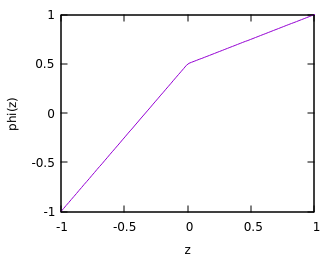
\includegraphics[width=7cm,keepaspectratio=true]{./Poisson.png}
 % Poisson.png: 0x0 pixel, 300dpi, 0.00x0.00 cm, bb=
 \caption{Illustration of the solution of the Poisson equation given by Eq.~\eqref{eq:poissonsol} for $\phi_0 = L = q = \varepsilon_0 = 1$.}
 \label{fig:poisson}
\end{figure}

In this section we will learn how to solve this equation numerically for an arbitrary charge distribution $\rho(z)$. Since it might be difficult to deal with $\delta$ distributions numerically, we shall consider, for instance, a Gaussian charge distribution $\rho(z) = q e^{-\frac{(z-z_0)^2}{2\Gamma^2}}$, where $z_0$ is the center of the distribution and $\Gamma$ is the broadening. For $z_0 = 0$ and small $\Gamma$ you should be able to reproduce the analytical solution above.


\subsection{The Sturm-Liouville problems}

In physics, many problems fall into differential equations that take the Sturm-Liouville form,

\begin{equation}
 \left\{\dfrac{d}{dx}\left[p(x) \dfrac{d}{dx}\right] + q(x)\right\}y(x) = \lambda w(x)y(x) + r(x),
 \label{eq:sturmliouville}
\end{equation}
where $p(x)$, $q(x)$, $w(x)$ and $r(x)$ are functions specified by the problem at hand, while $y(x)$ is the unknown function that we want to find. For instance, the Poisson equation in Eq.~\eqref{eq:poisson} is set by using $p(x) = 1$, $q(x) = w(x) = 0$, and $r(x) = -\rho(x)/\epsilon_0$. If $w(x) \neq 0$, $\lambda$ is the eigenvalue of the equation. We will discuss the class of eigenvalue problems later on in this Chapter, therefore, for now we shall take $w(x) = 0$. Moreover, let's assume that $p(x)$, $q(x)$ and $r(x)$ are analytical functions over the domain of interest.

Let's first present useful properties of the Sturm-Liouville equation without properly deriving them. For the derivations and more details please check specialized books on Mathematical Physics [refs] and Problem \ref{prob:sturmliouville}. Next, we use these properties to establish the Wronskian method to solve Sturm-Liouville problems.

\subsection*{The homogeneous Sturm-Liouville equation}

If $r(x) = 0$, Eq.~\eqref{eq:sturmliouville} is said homogeneous as it takes the form $\mathcal{L}y(x) = 0$, where $\mathcal{L}$ is the Sturm-Liouville operator, which is given by the terms between curly brackets, $\{\cdots\}$, in Eq.~\eqref{eq:sturmliouville}. It follows the properties:

\noindent
\textbf{(1) Principle of superposition.} Since this equation is linear, if $y_a(x)$ and $y_b(x)$ are solutions, then the linear combination $y_{c}(x) = a y_a(x) + b y_b(x)$ also satisfies $\mathcal{L}y_{c} = 0$. Here $a$ and $b$ are arbitrary constants that shall be defined by the boundary conditions, i.e. the linear combination coefficients.

\noindent
\textbf{(2) Linear independence.} Two solutions $y_a(x)$ and $y_b(x)$ are linearly independent if their Wronskian $W(x) \neq 0$ over the domain of $x$. The Wronskian of a pair of solutions $y_a(x)$ and $y_b(x)$ is $W(x) = y_a'(x) y_b(x) -y_b'(x)y_a(x)$. For the class of Sturm-Liouville homogeneous equations it is easy to show that 

\begin{equation}
 W(x) = W(x_0) \exp\left\{-\int_{x_0}^x \dfrac{p_1(x')}{p(x')}dx'\right\},
\end{equation}
where $p_1(x) = \frac{d}{dx} p(x)$, and $x_0$ belongs to the domain of $x$. Therefore, if the Wronskian $W(x_0) \neq 0$ in a specific point $x = x_0$, it will be non-zero over the whole domain.

\noindent
\textbf{(3) Uniqueness of the solution.} Since the Sturm-Liouville equation is a second-order ordinary differential equation, its solution is unique if it satisfies the ODE and two boundary (or initial) conditions. As a consequence, its most general solution can be written as a linear combination of two linearly independent solutions.

The properties above form the basis need to solve the homogeneous Sturm-Liouville problem using the Wronskian method. But before discussing this method, let's check the inhomogeneous Sturm-Liouville problem.

\subsection*{The inhomogeneous Sturm-Liouville equation}

For $r(x)\neq 0$ the Sturm-Liouville problem takes the form $\mathcal{L}y(x) = r(x)$, and is said to be inhomogeneous as it has a term independent of $y(x)$. In this case, the principle of superposition as stated above is not valid (see Problem \ref{prob:sturmliouville}). Instead, the generalized principle of superposition of inhomogeneous equations states that the most general solution can be written as

\begin{equation}
 y(x) = a y_a(x) + b y_b(x) + y_p(x),
 \label{eq:WronskianFull}
\end{equation}
where $y_a(x)$ and $y_b(x)$ are linearly independent solutions of the homogeneous equation $\mathcal{L}y_{a/b}(x) = 0$, and $y_p(x)$ is the particular solution of the inhomogeneous equation $\mathcal{L}y_p(x) = r(x)$. Here again, $a$ and $b$ are arbitrary constants to be set by the boundary conditions.

Since $y_a(x)$ and $y_b(x)$ are solutions of the homogeneous case, property \textbf{(2)} above follows and the Wronskian criteria can be used to verify or assure that $y_a(x)$ and $y_b(x)$ are linearly independent solutions. Property (3) also follows, and the solution $y(x)$ is unique if and only if it satisfies the ODE $\mathcal{L}y(x) = r(x)$ and the required boundary conditions.

\subsection{The Wronskian method}

The Wronskian method applies to both homogeneous and inhomogeneous cases of the Sturm-Liouville equation. Essentially, it provides a method to obtain a pair of linear independent solutions $y_a(x)$ and $y_b(x)$. We will state the problem for the inhomogeneous case, since the homogeneous case is simply a particular case in which $r(x) = 0$.

To guide our description let's consider Dirichlet boundary conditions, i.e. $y(x_0) = y_0$ and $y(x_1) = y_1$. Generalizations to Neumann or mixed boundary conditions will be simple enough and we leave it to the reader as an exercise. We want to solve the Sturm-Liouville equation $\mathcal{L}y(x) = r(x)$ in the domain $x_0 \leq x \leq x_1$.

\subsubsection{First step: find two linearly independent solutions of the homogeneous equation}

Our first step is to find a pair of linearly independent solutions $y_a(x)$ and $y_b(x)$ that satisfy the \textit{homogeneous} equation $\mathcal{L}y_{a/b}(x) = 0$. Accordingly to property \textbf{(2)} above, $y_a(x)$ and $y_b(x)$ will be linearly independent if their Wronskian $W(x) \neq 0$ at any point $x$. For practical purposes, we chose to analyze the Wronskian at $x = x_0$, the left end point of the domain. Namely, we want

\begin{equation}
 W(x_0) = y_a'(x_0)y_b(x_0) - y_a(x_0)y_b'(x_0) \neq 0.
\end{equation}

Notice that the final solution will be given by $y(x)$ in Eq.~\eqref{eq:WronskianFull}. Therefore the boundary conditions must apply to $y(x)$, and not to the auxiliary functions $y_a(x)$, $y_b(x)$ or $y_p(x)$. Therefore we can attribute auxiliary boundary conditions to $y_a(x)$ and $y_b(x)$ in order to assure that the condition above is satisfied and the pair $[y_a(x), y_b(x)]$ forms a set of linearly independent solutions. For instance, we may choose

\begin{align}
 y_a(x_0) &= 0, \text{  and  } y'_a(x_0) = A_1,\\
 y_b(x_0) &= A_2, \text{  and  } y'_b(x_0) = 0,
\end{align}
such that $W(x_0) = A_1 A_2$, where $A_1 \neq 0$ and $A_2 \neq 0$ are arbitrary nonzero constants.

The auxiliary boundary conditions above actually transforms the problem of finding $y_{a/b}(x)$ into a pair of independent \textbf{initial-value problems}, with the initial values for $y_a(x)$, $y_b(x)$ (and their derivatives) set above in terms of the arbitrary $A_1$ and $A_2$. We can use any initial-value problem method to obtain $y_{a/b}(x)$ satisfying the homogeneous equation $\mathcal{L}y_{a/b}(x) = 0$.

\subsubsection{Second step: find the particular solution of the inhomogeneous equation}

Now we need to find $y_p(x)$. Since this is also an auxiliary function, its boundary or initial conditions are arbitrary. Let's use $y_p(x_0) = B_1$ and $y'_p(x_0) = B_2$, where $B_1$ and $B_2$ are arbitrary constants. We can use any method of the initial-value problems to find $y_p(x)$.

\subsubsection{Third step: impose the physical boundary conditions}

In this final step we must impose the physical boundary conditions stated by our problem. Namely, we want $y(x_0) = y_0$ and $y(x_1) = y_1$. From Eq.~\eqref{eq:WronskianFull} we have

\begin{align}
 y(x_0) &= a y_a(x_0) + b y_b(x_0) + y_p(x_0) = b A_2 + B_1,\\
 y(x_1) &= a y_a(x_1) + b y_b(x_1) + y_p(x_1),
\end{align}
where $y_a(x_0) = 0$, $y_b(x_0) = A_2$, and $y_p(x_0) = B_1$ where the auxiliary initial conditions set above. The quantities $y_a(x_1)$, $y_b(x_1)$, and $y_p(x_1)$ are known from the solution of the auxiliary initial-value problems. To satisfy the boundary conditions, the coefficients $a$ and $b$ must be

\begin{align}
 b &= \dfrac{y_0-B_1}{A_2},\\
 a &= \dfrac{y_1 - b y_b(x_1) - y_p(x_1)}{y_a(x_1)}.
\end{align}

Combining these quantities, we have the all terms of Eq.~\eqref{eq:WronskianFull} to compose our final solution $y(x)$.

\subsubsection{Example: the Poisson equation via the Wronskian method}

Let's apply the Wronskian method to the Poisson equation to reproduce numerically the example of the beginning of this section; see Fig.~\ref{fig:poisson}. Let's write the Poisson equation, Eq.~\eqref{eq:poisson}, using the notation of the Sturm-Liouville problem above. It reads

\begin{equation}
 \dfrac{d^2}{dx^2} y(x) = -\rho(x).
\end{equation}
Next we use the ODE package to numerically find the auxiliary functions $y_a(x)$, $y_b(x)$ and $y_p(x)$ with appropriate initial conditions, and combine them at the end to satisfy the physical boundary condition.

The homogeneous version of the 1D Poisson's equation ($\rho(x) = 0$) is actually Laplace's equation in one dimension. Therefore it would be quite easy to find the solutions $y_a(x)$ and $y_b(x)$ of the homogeneous equation. It's simply $y_a(x) = (x-x_0)A_1$ and $y_b(x) = A_2$. However, in the numerical code below we choose to find these simple solutions numerically just to exemplify how to proceed in a more difficult scenario.

\begin{example}{Poisson via Wronskian method}
\label{ex:poissonWronskian}
\begin{minted}[mathescape,escapeinside=||]{julia}
using ODE
using PyPlot

z = linspace(-1.0, 1.0, 1000); # z axes
eps0 = 1.0; # $\varepsilon_0$

# charge density $\rho(z)$
g = 0.01; # broadening $\Gamma$
rho(z) = exp(-(z.^2)/(2*g^2))/(sqrt(2pi)*g);

# physical boundary conditions: $y_0$ and $y_1$
y0 = -1.0;
y1 = +1.0;

# find $y_a(z)$
A1 = 1.0;
ic = [0.0; A1]; # = (0, A1)
rhs(z, y) = [y[2]; 0.0];
za, ya = ode45(rhs, ic, z; points=:specified);
ya = map(k->k[1], ya);

# find $y_b(z)$
A2 = 1.0;
ic = [A2; 0.0]; # = (A2, 0)
rhs(z, y) = [y[2]; 0.0];
zb, yb = ode45(rhs, ic, z; points=:specified);
yb = map(k->k[1], yb);

# find $y_p(z)$
B1 = 0.0;
B2 = 0.0;
ic = [B1; B2]; # = (B1, B2)
rhs(z, y) = [y[2]; -rho(z)/eps0];
zp, yp = ode45(rhs, ic, z; points=:specified);
yp = map(k->k[1], yp);

# coefficients and final solution
b = (y0 - B1)/A2;
a = (y1 - b*yb[end] - yp[end])/ya[end];
y = a*ya + b*yb + yp;

plot(z, y);
\end{minted}
\end{example}

\subsection{Schroedinger equations: transmission across a barrier}

Let's consider a free electron in one dimension colliding with a general shaped barrier set by a potential $V(x)$. The dynamics of this electron is tunnel or scatter back as it collides with the barrier. Here we want to calculate the transmission $T$ and reflection $R$ probabilities.

The Hamiltonian of the system is

\begin{equation}
 H = -\dfrac{1}{2}\dfrac{\partial^2}{\partial x^2} + V(x).
\end{equation}
Here we use atomic units ($\hbar = 1$, $m=1$), and $V(x)$ is a general potential within the scattering region $0 \leq x \leq L$, and $V(x) = 0$ outside these limits.

Referring to the region $x<0$ as I, let's assume that the state of the electron is a linear combination of the injected and reflected waves,

\begin{equation}
 \psi_I(x) = e^{i k x} + r e^{-i k x},
 \label{eq:psi1}
\end{equation}
where $r$ the reflection coefficient, and $k = \sqrt{2\varepsilon}$ and $\varepsilon$ is the electron energy.

We'll refer to the region $x>L$ as III. There the electron state is composed solely by the transmitted wave,

\begin{equation}
 \psi_{III}(x) = t e^{ikx},
 \label{eq:psi3}
\end{equation}
where $t$ is the transmission coefficient.

At the central region (II), where $0 \leq x \leq L$, we need to find two linear independent solutions, $\psi_a(x)$ and $\psi_b(x)$, of the Schroedinger equation $H\psi(x) = \varepsilon\psi(x)$. I'll leave this as a Problem for the reader. These solutions can be combined in a general linear combination

\begin{equation}
 \psi_{II}(x) = a \psi_a(x) + b \psi_b(x),
 \label{eq:psi2}
\end{equation}
where $a$ and $b$ are the linear combination coefficients.

The final solution and its derivative must be continuous at the interfaces $x=0$ and $x=L$. Therefore, we impose the conditions: (i) $\psi_I(0) = \psi_{II}(0)$; (ii) $\psi'_I(0) = \psi'_{II}(0)$; (iii) $\psi_{II}(L) = \psi_{III}(L)$; (iv) $\psi'_{II}(L) = \psi'_{III}(L)$. These give us the following equation for the coefficients $a$, $b$, $r$ and $t$:

\begin{equation}
 \begin{pmatrix}
  \psi_a(0) & \psi_b(0) & -1 & 0 \\
  \psi'_a(0) & \psi'_b(0) & ik & 0 \\
  \psi_a(L) & \psi_b(L) & 0 & e^{ikL}\\
  \psi'_a(L) & \psi'_b(L) & 0 & ike^{ikL}
 \end{pmatrix}
 \begin{pmatrix}
  a \\ b \\ r \\ t
 \end{pmatrix}
 =
 \begin{pmatrix}
  1 \\ ik \\ 0 \\ 0
 \end{pmatrix}.
 \label{eq:psimatch}
\end{equation}

From the equation above one can easily extract $t$. The transmission probability is then $T = |t|^2$, and the reflection probability is $R = |r|^2$. You can check that $T+R=1$.

In Fig.~\ref{fig:transmission} we consider the transmission over a Gaussian barrier

\begin{equation}
 V(x) = e^{-\frac{1}{2}(x-x_0)^2},
\end{equation}
where $x_0 = L/2$ is the center of the barrier, and $L = 20$.

\begin{figure}[ht!]
 \centering
 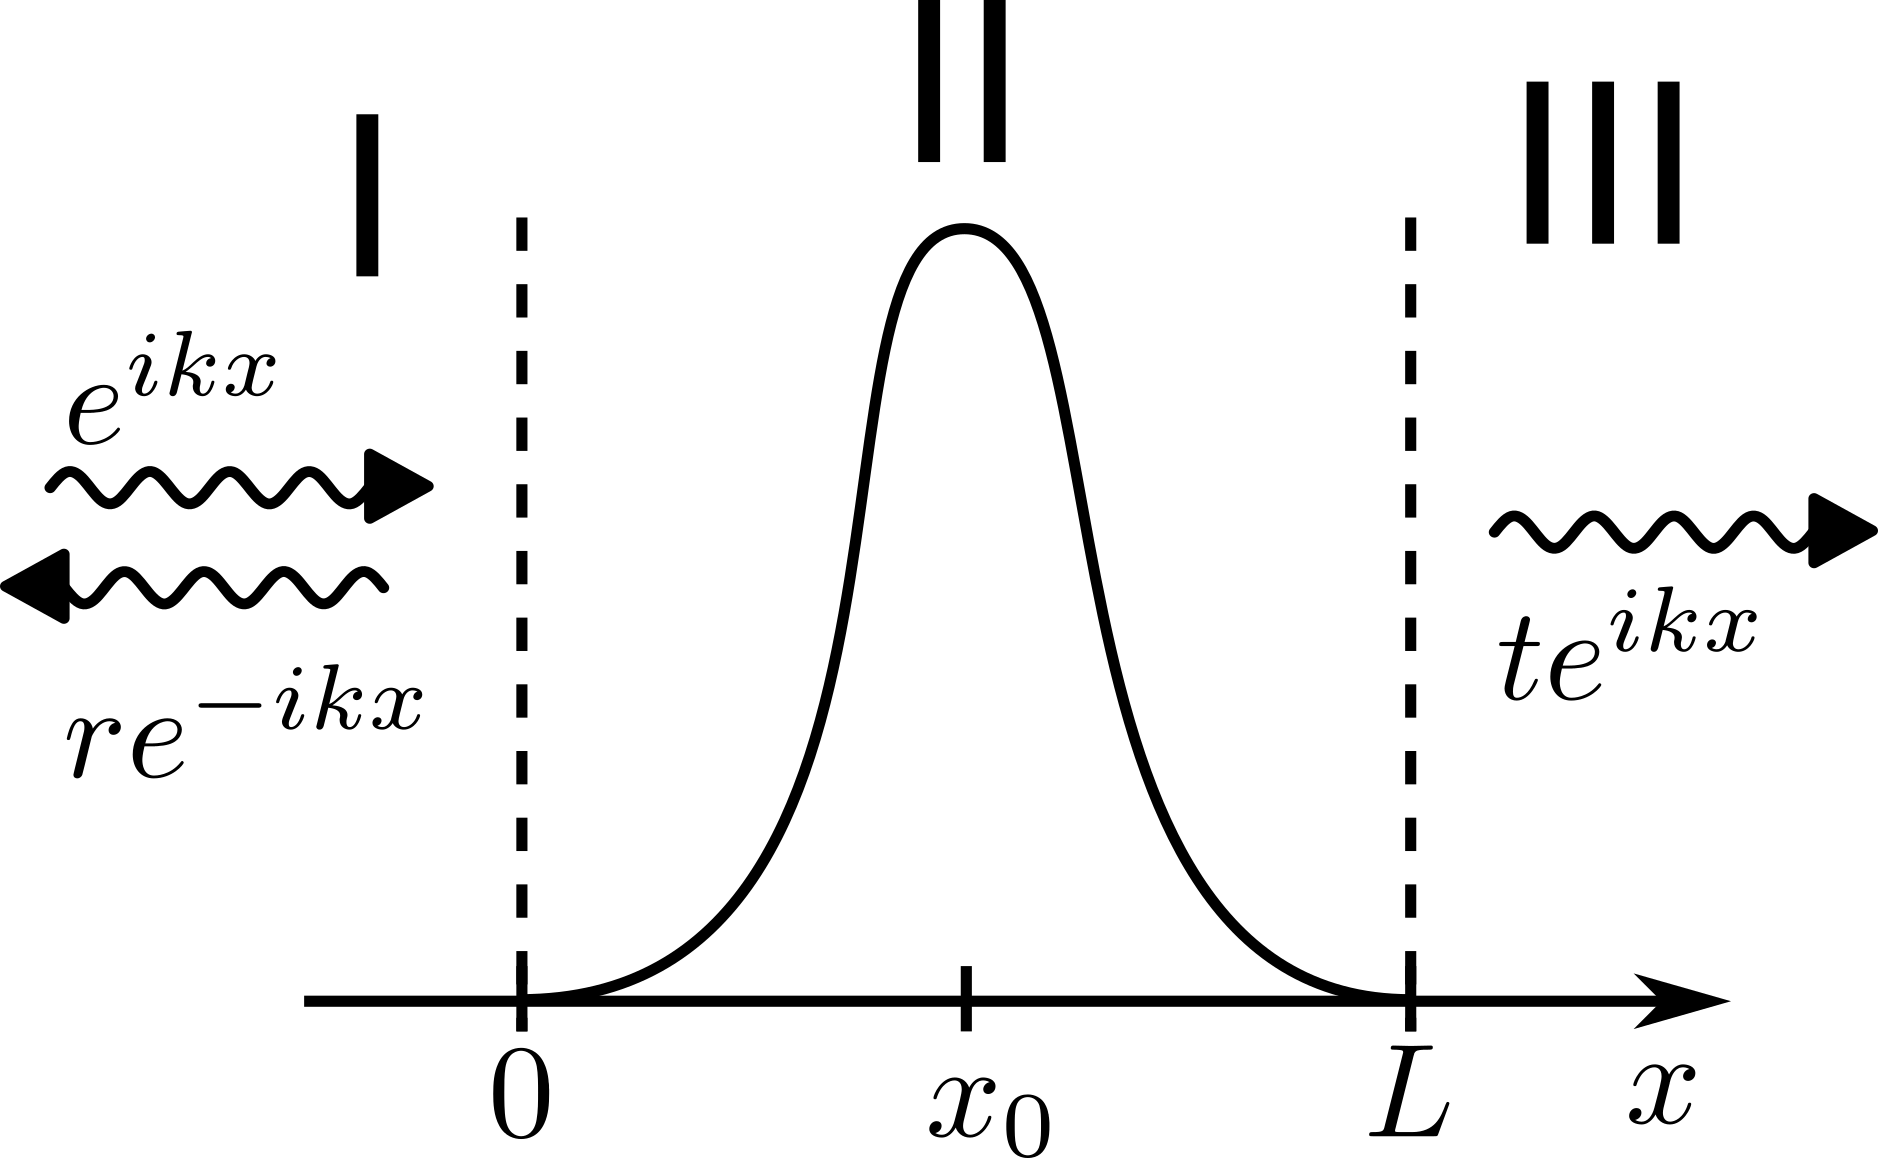
\includegraphics[width=0.45\columnwidth]{./transmissionbarrier.png}
 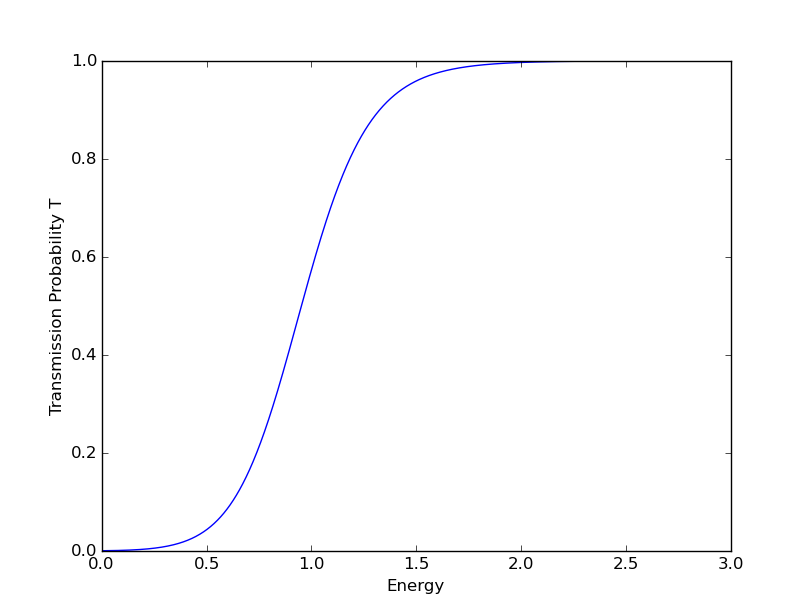
\includegraphics[width=0.45\columnwidth]{./transmission.png}
 % transmission.png: 0x0 pixel, 300dpi, 0.00x0.00 cm, bb=
 \caption{(left) Illustration of the Gaussian barrier with the injected, reflected and transmitted waves at outer regions. (right) Transmission probability $T$ as a function of the energy $\varepsilon$.}
 \label{fig:transmission}
\end{figure}


\subsection{Non-linear differential equations}

For non-linear differential equations, the properties of Sturm-Liouville operator discussed in the previous sections does not hold. Particularly, there is no superposition principle for non-linear ODEs. As a consequence, the task to solve a boundary value problem for a non-linear ODE can be quite difficult.

The non-linearity implies that a ODE with a specific set of boundary conditions may have more than one solution. This is again in direct contrast with the Sturm-Liouville case, where the uniqueness theorem (by Picard–Lindelöf) states that given the boundary or initial conditions, the ODE has only one solution.

Let's illustrate this with a very simple differential equation:

\begin{equation}
 \dfrac{d^2 y(x)}{dx^2} + |y(x)| = 0,
\end{equation}
which is non-linear due to the absolute value in the second term. Consider that the boundary conditions are $y(0) = 0$ and $y(4) = -2$.

\subsubsection{The shooting method}

One way of solving this problem is the shooting method. First, convert the second order differential equations into a pair of coupled first order differential equations. This is the same procedure used at the begging of this chapter. We know how to solve initial value problems easily. Therefore, consider the auxiliary initial conditions $y(0) = y_0$ and $y'(0) = v_0$. Clearly, it is useful to set $y_0 = 0$ to automatically satisfy our desired boundary condition. The problem is $v_0$. What is the appropriate value of $v_0$ that satisfies our boundary conditions? Namely, we want $v_0$ set such the evolution of the initial value problem yields $y(4) = -2$.

In the general there's no direct approach to find the appropriate value of $v_0$. In our example there's actually two possible values of $v_0$ that yield $y(4) = -2$. To see this, I invite the reader to write a code using the Runge-Kutta method, or Julia's ODE package to solve the initial value problem for the example above for different values of the initial condition $y'(0) = v_0$. Evolving the solution from $x=0$ to $x=4$ we can extract $y(4)$ for each value of $v_0$ and plot $y(4) \times v_0$. This is shown in Fig.~\ref{fig:shooting}.


\begin{figure}[ht!]
 \centering
 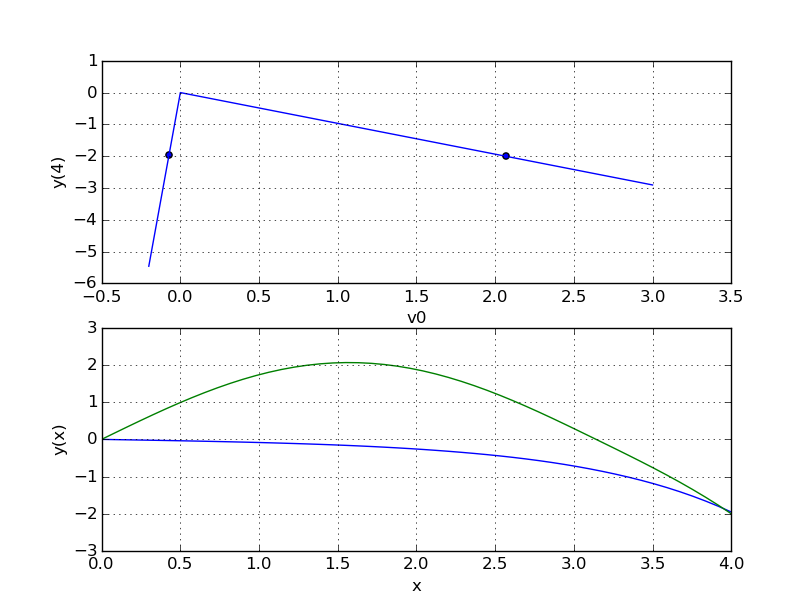
\includegraphics[width=0.70\columnwidth]{./shooting.png}
 % transmission.png: 0x0 pixel, 300dpi, 0.00x0.00 cm, bb=
 \caption{(top) Values of $y(4)$ obtained propagating the non-linear differential equation from $x=0$ to $x=4$ with the initial condition set to $y'(0) = v_0$, as a function of $v_0$. There are two values of $v_0$ that satisfy $y(4) = -2$, as indicated by the circles.
 (bottom) The two possible solutions $y(x) \times x$ for the values of $v_0$ found to satisfy the boundary conditions. }
 \label{fig:shooting}
\end{figure}

\section{The eigenvalue problem}

Here we'll consider only eigenvalue problems of linear and homogeneous differential equations. Particularly, we are only interest again in the Sturm-Liouville problems. In the Sturm-Liouville Eq.~\eqref{eq:sturmliouville}, the differential equation is an eigenvalue problem if $w(x) \neq 0$ and $r(x) = 0$. Therefore we have

\begin{equation}
 \left\{\dfrac{d}{dx}\left[p(x) \dfrac{d}{dx}\right] + q(x)\right\}y(x) = \lambda w(x)y(x),
\end{equation}
where $p(x)$, $q(x)$ and $w(x)$ are given functions set by the problem at hand, while $\lambda$ and $y(x)$ are the unknowns that we want to find. For a set of boundary conditions, this differential equation have solutions only for particular values of $\lambda$, which are called the eigenvalues. The solutions $y(x)$ associated with each particular $\lambda$ are the eigenfunctions. If we vectorize this equation using finite differences, the function $y(x)$ becomes a vector: the eigenvector.

There are many ways of solving an eigenvalue problem numerically. But let's first check two analytical cases to serve as examples where we can try our numerical approaches.

\subsection{Oscillations on a string}

A string fixed at its end points separated by a distance $\ell$ satisfy the wave equation,

\begin{equation}
 \dfrac{\partial^2 y(x,t)}{\partial x^2} - \dfrac{1}{v^2} \dfrac{\partial^2 y(x,t)}{\partial t^2} = 0,
\end{equation}
where $y(x,t)$ is the string profile as a function of space $x$ and time $t$, and $v$ is the wave velocity on the string. This is a partial differential equation, but in this chapter we are dealing with ordinary differential equations only. Since for now we are only interested in the normal modes of oscillation, we can Fourier transform the equation from time $t$ to frequency $w$, yielding

\begin{equation}
 \dfrac{\partial^2 y(x,\omega)}{\partial x^2} + \dfrac{\omega^2}{v^2} y(x,\omega) = 0.
\end{equation}
This equation takes the form of eigenvalue Sturm-Liouville problem if we set $p(x) = 1$, $q(x) = 0$, $w(x) = 1$, and $\omega^2 = v^2 \lambda$.

If the string is fixed at its end points, the boundary conditions are $y(0,t) = 0$, and $y(\ell,t) = 0$ for any $t$. Equivalently, the Fourier transformed $y(x,\omega)$ also satisfy the same boundary conditions: $y(0, \omega) = 0$ and $y(\ell, \omega) = 0$ for any $\omega$.

You have probably seen already in a theoretical physics class that the solution to this problem is

\begin{equation}
 y(x,\omega_n) = A \sin\left(\dfrac{\omega_n}{v} x\right),
\end{equation}
where $k_n = \omega_n/v$ are the quantized wave-numbers, $\omega_n = n \pi v/\ell$ are the quantized frequencies, and the integer $n$ labels the normal modes of oscillation. The amplitude $A$ depends on the initial condition, which we will not consider yet.

\subsection{Electron in a box}

An electron in a box is described by the Schroedinger equation. It's dynamics is set by the time-dependent Schroedinger equation. But similarly to the string oscillations, its normal modes are given by a static equation, the time-\textit{independent} Schroedinger equation,

\begin{equation}
 -\dfrac{1}{2}\dfrac{\partial^2}{\partial x^2} \psi(x) + V(x) \psi(x) = \varepsilon \psi(x),
 \label{eq:Schroedinger}
\end{equation}
where we use atomic units ($\hbar = 1$, $m=1$) for simplicity. Here $V(x)$ is the electrostatic potential that confines the electron, $\psi(x)$ is the wave-function and $\varepsilon$ is the energy. This is indeed a Sturm-Liouville eigenvalue problem where the eigenvalue is the energy $\varepsilon$ and the eigenfunction is the wave-function $\psi(x)$.

If the electron is trapped in a box of width $\ell$ with hard walls, such that $V(x) = 0$ for $0 < x < \ell$, and $V(x) = \infty$ outside, the wave-function must satisfy the boundary-conditions $\psi(0) = 0$ and $\psi(\ell) = 0$.

Since $V(x) = 0$ inside the box, the problem is very similar to the oscillations on a string. The solutions are

\begin{equation}
 \psi_n(x) = A \sin(k_n x),
 \label{eq:psin}
\end{equation}
where the wave-numbers $k_n = n\pi/\ell$, the eigenenergies $\varepsilon_n = \frac{1}{2}k_n^2$, and the integer $n$ labels the quantized eigenstates of the electron.

\subsection{Method of finite differences}

For simplicity let's consider the Sturm-Liouville eigenvalue problem with $p(x) = 1$ and $w(x) = 1$,

\begin{equation}
 \left\{\dfrac{d^2}{dx^2} + q(x)\right\}y(x) = \lambda y(x).
\end{equation}

We have seen in Chapter \ref{sec:matrixrepresentation} that we can represent the derivative operators as matrices. Particularly, the second derivative becomes

\begin{equation}
\dfrac{d^2}{dx^2}y(x) = 
 \begin{pmatrix}
  y''_1 \\y''_2 \\ y''_3 \\ y''_4 \\ \cdots \\ y''_i \\ \cdots \\ y''_{N-1} \\ y''_N
 \end{pmatrix}
 = \dfrac{1}{h^2}
\begin{pmatrix} 
 -2 & 1 & 0 & 0 & 0 & 0 & 0 & 0 & 0\\
 1 & -2 & 1 & 0 & 0 & 0 & 0 & 0 & 0\\
 0 & 1 & -2 & 1 & 0 & 0 & 0 & 0 & 0\\
 0 & 0 & 1 & -2 & 1 & 0 & 0 & 0 & 0\\
 0 & 0 & 0 & 1 & -2 & 1 & 0 & 0 & 0\\
 0 & 0 & 0 & 0 & 1 & -2 & 1 & 0 & 0\\
 0 & 0 & 0 & 0 & 0 & 1 & -2 & 1 & 0\\
 0 & 0 & 0 & 0 & 0 & 0 & 1 & -2 & 1\\
 0 & 0 & 0 & 0 & 0 & 0 & 0 & 1 & -2
\end{pmatrix}
\begin{pmatrix}
  y_1 \\y_2 \\ y_3 \\ y_4 \\ \cdots \\ y_i \\ \cdots \\ y_{N-1} \\ y_N
\end{pmatrix},
\end{equation}
where $y_i = y(x_i)$ and $x_i$ are the discretized coordinates.
I leave as an exercise to the reader to check that this representation is compatible with the boundary conditions $y(0) = 0$ and $y(\ell) = 0$. Here the discretization of $x$ is such that $x_0 = 0$ and $x_{N+1} = \ell$, and $h$ is the discrete step.

The $q(x)$ term is local, therefore its matrix representation is diagonal,

\begin{equation}
q(x)y(x) = 
\begin{pmatrix}
 q_1 & 0 & 0 & 0 & 0 & 0 & 0 & 0 & 0\\
 0 & q_2 & 0 & 0 & 0 & 0 & 0 & 0 & 0\\
 0 & 0 & q_3 & 0 & 0 & 0 & 0 & 0 & 0\\
 0 & 0 & 0 & q_4 & 0 & 0 & 0 & 0 & 0\\
 0 & 0 & 0 & 0 & \ddots & 0 & 0 & 0 & 0\\
 0 & 0 & 0 & 0 & 0 & q_i & 0 & 0 & 0\\
 0 & 0 & 0 & 0 & 0 & 0 & \ddots & 0 & 0\\
 0 & 0 & 0 & 0 & 0 & 0 & 0 & q_{N-1} & 0\\
 0 & 0 & 0 & 0 & 0 & 0 & 0 & 0 & q_N
\end{pmatrix}
\begin{pmatrix}
  y_1 \\y_2 \\ y_3 \\ y_4 \\ \cdots \\ y_i \\ \cdots \\ y_{N-1} \\ y_N
\end{pmatrix}.
\end{equation}
where $q_i = q(x_i)$.

With these matrix representations, the differential equation above can be put in a matrix form $H y = \lambda y$. The matrix $H$ is the sum of matrices above, $y$ is the vector composed by $y_i$, and $\lambda$ is the eigenvalue.

The most used numerical package to solve eigenvalue problems in a matrix form is Lapack\footnote{Lapack: \url{http://www.netlib.org/lapack/}}. The language Julia has this package natively implemented in the command \texttt{eig}. Try to run the next example.

\begin{example}{Eigenvalues and eigenvectors}
\label{ex:eig}
\begin{minted}[mathescape,escapeinside=||]{julia}
using PyPlot

# creates the matrix $H = -\partial_x^2$
H = 2*diagm(ones(10)) - diagm(ones(9),1) - diagm(ones(9),-1);

# calculates the eigenvalues and eigenvetors
evals, evecs = eig(H);

subplot(311)
plot(evecs[:,1]) # plot the first eigenvector

subplot(312)
plot(evecs[:,2]) # plot the second eigenvector

subplot(313)
plot(evecs[:,3]) # plot the third eigenvector

# print the first three eigenvalues
println("E1 = ", evals[1]);
println("E2 = ", evals[2]);
println("E3 = ", evals[3]);

\end{minted}
\end{example}

As you can see in the example, the \texttt{eig} command receives the matrix $H$ and returns its eigenvalues in a vector and the eigenvetors as a matrix. In this eigenvector matrix, each eigenvector is set as a column. Therefore \texttt{evecs[:,n]} returns the eigenvetor $n$.

\section{Problems}

\begin{problem}{Damped harmonic oscillator}
 \label{prob:damped}

 Implement a code to solve the damped harmonic oscillator problem,
 
 \begin{equation}
  \dfrac{d^2 x(t)}{dt^2} = -\omega_0^2 x(t) - \gamma \dfrac{dx(t)}{dt}.
 \end{equation}
 Fix $\omega_0 = 2\pi$ and solve the equation for different values of $\gamma$ to show the solutions for the three possible regimes: (i) subcritical; (ii) critical; and (iii) supercritical. You will find the exact solutions on the volume 2 of Ref.~\cite{nussenzveig2007curso}.
\end{problem}

\begin{problem}{Compare Euler and RK for the pendulum}
 \label{prob:compareEulerRK}
 
 Compare the results of Example \ref{ex:euler} and Example \ref{ex:odependulum} for small and large time steps \texttt{tau}, and for small and large oscillations (amplitude \texttt{x0}).
\end{problem}

\begin{problem}{Runge Kutta RK4}
 \label{prob:rk4}
 
 Implement your own version of the RK4 code in Julia to solve the pendulum problem or any other different equation you may prefer. Your code won't be more efficient than the adaptive code in the ODE package. However it is a good practice for you to implement the RK4 by yourself, since it is the most well known and used method for differential equations.
\end{problem}

\begin{problem}{Sturm-Liouville equation}
 \label{prob:sturmliouville}

 \textbf{Tip:} Check Moysés Nussenzveig's book, volume 2, chapter on oscillations \cite{nussenzveig2007curso}.
 
 (a) Derive the three properties listed for the homogeneous Sturm-Liouville problem: (1) principle of superposition; (2) linear independence; and (3) Uniqueness of the solution.
 
 (b) Derive the generalization of the principle of superposition for inhomogeneous equations.
  
\end{problem}

\begin{problem}{Wronskian}
 \label{prob:Wronskian}

 (a) Show that for an homogeneous Sturm-Liouville differential equation the Wronskian $W(x) = y'_a(x)y_b(x)-y_a(x)y'_b(x)$ can be written as
 
\begin{equation}
 W(x) = W(x_0) \exp\left\{-\int_{x_0}^x \dfrac{p_1(x')}{p(x')}dx'\right\},
\end{equation}

 (b) Show that if the Wronskian is nonzero over the whole domain, the solutions $y_a(x)$ and $y_b(x)$ are linearly independent. 
 
\end{problem}


\begin{problem}{Quantum transmission probability for electrons}
 
 (a) Why do we identify the positive exponentials in $\psi_I(x)$ and $\psi_{III}(x)$, Eqs.~\eqref{eq:psi1}-\eqref{eq:psi3}, as forward moving, and the negative one as a backwards motion?
 
 (b) Show that matching the continuity conditions at the interfaces $x=0$ and $x=L$ leads to Eq.~\eqref{eq:psimatch}.
 
 (c) Implement a code using the Wronskian method to obtain $\psi_a(x)$ and $\psi_b(x)$ and calculate $t$.
 
 (d) Transform the code of item (c) into a function that receives the energy $\varepsilon$ and returns the transmission $T = |t|^2$. Use this code to reproduce the transmission probability plot shown in Fig.~\ref{fig:transmission}.
 
 (e) Try now with two Gaussian barriers, and run for a thin energy grid. You will see the Fabry–Pérot resonances at the quasi-confined states of a resonant-tunneling diode.
 
\end{problem}


\begin{problem}{The Schroedinger equation and the Sturm-Liouville parameters}
 
 (a) What are the expressions for the Sturm-Liouville parameters $p(x)$, $q(x)$, $w(x)$ and $r(x)$ that represents the time-independent Schroedinger equation, Eq.~\eqref{eq:Schroedinger}? 
 
 (b) Show that the solution of electron in a box problem is given by Eq.~\eqref{eq:psin} with eigenenergies $\varepsilon_n = \frac{1}{2}(n\pi/\ell)^2$.
 
\end{problem}


\begin{problem}{Matrix representation of the derivative operator}
 
 (a) The matrix representation of the derivative operator using finite differences faces a problem at the edges. Show that this is not a problem when we consider hard wall boundary conditions: $y(0) = 0$ and $y(\ell) = 0$.
 
 (b) What changes in the matrix representation if we consider periodic boundary conditions? Namely $y(\ell) = y(0)$.
 
\end{problem}


\begin{problem}{The potential well}

  (a) Implement a code to solve the time-independent Schroedinger equation for a Gaussian potential well,
  
  \begin{equation}
   V(x) = V_0 e^{-\frac{1}{2}(x-c)^2},
  \end{equation}
  with amplitude $V_0 = -10$, centered at $c = \ell/2$, hard-wall boundary conditions $\psi(0) = \psi(\ell) = 0$, and $\ell = 10$.
  
  (b) Make a plot of the potential well and the first three eigenstates.
  
  (c) Compare the solution with a discretization of $x$ with 100 points and with 500 points. The result (eigenvalues and eigenvectors) must not change much if the implementation is correct.
 
\end{problem}






